%
% The first command in your LaTeX source must be the \documentclass command.
\documentclass[sigchi]{acmart}

%
% defining the \BibTeX command - from Oren Patashnik's original BibTeX documentation.
\def\BibTeX{{\rm B\kern-.05em{\sc i\kern-.025em b}\kern-.08emT\kern-.1667em\lower.7ex\hbox{E}\kern-.125emX}}

% Rights management information.
% These commands are for a PROCEEDINGS abstract or paper.
\copyrightyear{2026}
\acmYear{2026}
\setcopyright{acmlicensed}
\acmConference[SNA '26]{Social Network Analysis '26}{2025/26}{University of Pisa, Italy}
\acmBooktitle{Social Network Analysis '26}
\acmPrice{0.00}
\acmDOI{}
\acmISBN{}
\setlength{\skip\footinscopyrightpermission}{8pt}
\settopmatter{printacmref=false}

% Additions to the template: figures side by side, tables that never exceed the column, folder of the figures
\usepackage{subcaption}
\usepackage{adjustbox}
\graphicspath{{img/}{../figures/}}
\emergencystretch=1.5em

% end of the preamble, start of the body of the document source.
\begin{document}

\title[Geography of the Core]{Geography of the Core: Centrality and Participation in the Horizon Europe Collaboration Network}

\author{Giulia Rossi}
\email{g.rossi142@studenti.unipi.it}
\affiliation{%
  \institution{Student ID: 694076}
}

\renewcommand{\shortauthors}{G. Rossi}

\begin{abstract}
Collaborative projects funded by the Framework Programmes of the European Union connect organisations of different countries into a large collaboration network. This work examines whether the most central organisations in the communities of the Horizon Europe network are evenly distributed across geographic areas. It then asks whether differences in centrality between areas remain among organisations with the same number of projects, that is, whether the organisations of some areas are less central than their participation alone would imply. The network was built from CORDIS data (35,200 organisations, 1,061,382 links) and communities were detected with the Louvain algorithm. The analysis was then repeated on a null model that reassigns partners at random while preserving the participation of every organisation. The results show that the central organisations are unevenly distributed across areas. Most of this imbalance, however, mirrors differences in participation: organisations with a similar number of projects are similarly central wherever they are based, with few exceptions at the level of single countries.
\footnote{
{\bf Project Repository}\\
\noindent Data collection, analytical tasks and report: \url{https://github.com/grossi42/2026_rossi}}
\end{abstract}

\keywords{Social Network Analysis, Collaboration Networks, Community Discovery, Centrality, Horizon Europe}

\maketitle
\bigskip
\section{Introduction}

The Framework Programmes are the programmes through which the European Union funds research and innovation, and many of the projects they support are collaborative: consortia of organisations from different countries apply for a grant and carry out the work together. Horizon Europe, the ninth programme, runs from 2021 to 2027 with an overall budget of about 95.5 billion euros~\cite{regulation,ep2021}. Every funded consortium records a choice of partners, and the network formed by these choices has been studied since the early programmes. In the first five programmes it showed heavy-tailed degree distributions and short distances, with very similar features from one programme to the next, and a stable core of interlinked organisations, mostly universities and research centres~\cite{roediger2008}, whose centrality strengthened over time~\cite{breschi2004}.

A second feature is just as persistent, and it is geographic. Horizon Europe includes a specific part, \emph{Widening participation and strengthening the European Research Area}, whose actions are coordinated by organisations from the countries with lower research and innovation performance: fifteen Member States, a group of associated countries and the outermost regions~\cite{regulation,widening}. In the earlier programmes, the newer Member States became more integrated into the network over time, but remained more involved in the less complex parts of the programmes~\cite{balland2019}.

What these differences mean for the collaboration network is less clear, and two readings are possible. In the first, organisations from these countries simply take part in fewer projects: the disadvantage lies in \emph{participation}. In the second, they end up at the margins of the collaboration structure when they do take part: the disadvantage lies in \emph{position}. The two readings call for different responses, and counting projects alone cannot tell them apart. Comparing organisations with the same number of projects can. This work therefore addresses the following question:

\begin{quote}
\textbf{RQ.} In the communities of the Horizon Europe collaboration network, are the most central organisations evenly distributed across geographic areas? If not, is the difference explained by the number of projects each organisation takes part in, or does it remain when comparing organisations with the same number of projects?
\end{quote}

Answering it requires care, because the network is the projection of a bipartite structure: every project links all its participants to each other. Dense groups and high clustering therefore arise mechanically, whoever collaborates with whom, and organisations that take part in many or large projects accumulate partners by construction~\cite{newman2001,opsahl2013}. A theme that runs through this report is that much of what looks like structure in such a network is produced by its construction, and that a conclusion is only as sound as the baseline it is compared with.

The report follows the project brief. Section~\ref{sec:data} describes how the data were collected from CORDIS and how the network was built. Section~\ref{sec:analysis} characterises its topology against Erd\H{o}s--R\'enyi and Barab\'asi--Albert graphs, and shows where these standard references fall short for our data. Section~\ref{sec:open} addresses the research question with a null model that keeps the projects, the size class of every project and the participation of every organisation, and randomises only the partners. Section~\ref{sec:discussion} discusses the answer, its policy reading and its limits.

\section{Data Collection}
\label{sec:data}

\subsection{Selected Data Source}

Data come from CORDIS, the European Commission's public repository of EU-funded research projects, through the bulk exports that the Publications Office of the EU releases every month on the EU Open Data Portal~\cite{cordis}. We use the Horizon Europe dataset in its version of 28 September 2026.

Two tables are extracted. The \emph{participations}, taken from the CSV export, record which organisations take part in which projects: each row is one organisation in one project, with its identifier, name, country, activity type and role in the consortium.  The \emph{projects} are rebuilt from the JSON export, which has one file per project, keeping the identifier and the start date. The project table of the CSV export was discarded: unescaped quotes inside its text fields break the structure of some rows, so that a standard parser stops with an error and a tolerant one loses part of the projects.

\subsection{Collection Methodology and Assumptions}

{\sloppy Data collection is scripted. Two archives are downloaded by the notebook \texttt{01\_\allowbreak data\_\allowbreak collection.ipynb}, which stores the two tables in \texttt{data/\allowbreak snapshot}. Since CORDIS updates its exports every month, all later steps read this stored copy, and the results do not depend on when the data are downloaded again.\par}

The data describe a bipartite network, in which organisations take part in projects, but this study focuses on its projection onto the organisations. Each of the 35,200 organisations that take part in at least one project is a node. Two organisations are linked when they have worked on at least one project together, and the weight of the link counts the projects they share. Every node carries four attributes: its country, its activity type (higher education, research organisation, private company, public body or other), the number of projects it takes part in and the number it coordinates.

The projection rests on four design choices, which we state because each of them shapes the network.

\emph{Roles.} CORDIS records four roles: coordinator, participant, associated partner (a member of the consortium that receives no EU funding) and third party. All four generate links, since all of them take part in the work of the project. Had the network been restricted to the beneficiaries of the grant, coordinators and participants, 21\% of the participations would have been discarded.

\emph{Duplicates.} In 278 cases the same organisation appears twice in the same project, and in 230 of them with two different roles. Each pair is counted only once, and an organisation listed as coordinator in either record keeps that role.

\emph{Status and dates.} Every project in the snapshot is included, whatever its status or start date, and so are participations that ended early. A link therefore means that two organisations took part in the same project, whether or not the project is still running.

\emph{Single-participant projects.} A project with one participant creates no link. Organisations that take part only in such projects are kept in the network as isolated nodes, since they too belong to the population the programme funds.

\subsection{Data Characterization}

\begin{table}[t]
\caption{The dataset and the network built from it.}
\label{tab:data}
\small
\setlength{\tabcolsep}{4pt}
\begin{adjustbox}{max width=\columnwidth}
\begin{tabular}{lr}
\toprule
Projects & 23,613 \\
\quad with at least two participants & 12,541 (53.1\%) \\
Participations (organisation--project pairs) & 145,631 \\
Organisations (nodes) & 35,200 \\
Links (edges) & 1,061,382 \\
\quad with weight above 1 & 132,549 (12.5\%) \\
Isolated organisations & 818 (2.3\%) \\
Giant component (nodes) & 34,271 (97.4\%) \\
Average degree & 60.3 \\
Density & 0.0017 \\
\bottomrule
\end{tabular}
\end{adjustbox}
\end{table}

\begin{figure*}[t]
\centering
\begin{subfigure}{0.32\textwidth}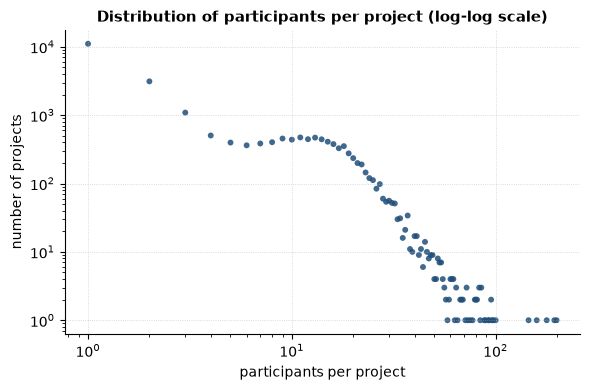
\includegraphics[width=\linewidth]{participants_per_project.png}\end{subfigure}\hfill
\begin{subfigure}{0.32\textwidth}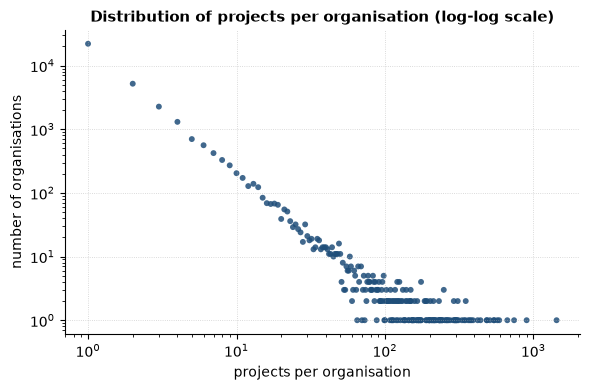
\includegraphics[width=\linewidth]{projects_per_organisation.png}\end{subfigure}\hfill
\begin{subfigure}{0.32\textwidth}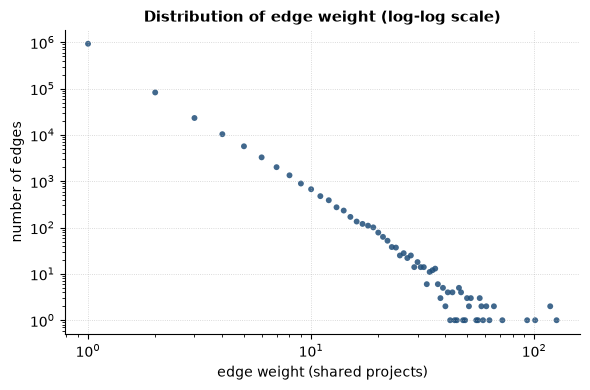
\includegraphics[width=\linewidth]{edge_weight_distribution.png}\end{subfigure}
\caption{The three skewed distributions behind the network: size of the consortia (left), activity of the organisations (centre) and weight of the links (right).}

\label{fig:data}
\end{figure*}

Two of these distributions shape much of what follows (Figure~\ref{fig:data}). The first is the size of the consortia. Almost half of the projects (46.9\%) have a single participant, as in individual grants and fellowships, and generate no link. Among the others, sizes range up to 199 participants. Since each of its $n$ participants is linked to all the others, a project yields $n(n-1)/2$ pairs, a number that grows far faster than the consortium itself: the largest 1\% of the projects alone produce 30.4\% of all pairs. The second is the activity of the organisations: 62.6\% take part in a single project, while the most active one takes part in 1,432, and the top 1\% account for 35.1\% of all participations.

The population, moreover, is not quite what the phrase ``research network'' may suggest. Private companies make up 58\% of the organisations, whereas universities and research organisations together account for only 18\%. Geography is concentrated as well: four countries alone, namely Germany, Spain, France and Italy, host 36\% of the organisations. The attributes, on the other hand, are virtually complete, with the country missing for five organisations and the activity type for just one. Coverage in time is uneven by design. Between roughly 3,300 and 5,100 projects start in each year from 2022 to 2026, while 932 projects already signed will only start in 2027. The most recent years are therefore still incomplete.

Once projected, the 1,335,249 pairs generated by the projects collapse into 1,061,382 distinct links, since many organisations meet more than once: 12.5\% of the links join organisations that share several projects, up to as many as 126 (Table~\ref{tab:data}). The resulting network is almost entirely connected: a single giant component gathers 97.4\% of the nodes, leaving aside only 45 small components and 818 isolated organisations. These are far fewer than the share of single-participant projects might suggest, and for a simple reason: an organisation is isolated only if every one of its projects is of that kind.

\section{Network Characterization}
\label{sec:analysis}

As the brief requires, the network is examined in its simplest form, undirected and unweighted, and measured against two benchmarks: an Erd\H{o}s--R\'enyi (ER) graph with the same number of nodes and links~\cite{erdos1959}, and a Barab\'asi--Albert (BA) graph with the same number of nodes and $m = 30$ links per new node~\cite{barabasi1999}. All measures are computed with \texttt{igraph}~\cite{igraph}. Distances and centralities, however, are confined to the giant component of each network, which in CORDIS leaves out only a small fringe of organisations. Table~\ref{tab:summary} gathers the results.

\begin{table}[t]
\caption{The Horizon Europe network (CORDIS) and the two reference models.}
\label{tab:summary}
\small
\setlength{\tabcolsep}{4pt}
\begin{adjustbox}{max width=\columnwidth}
\begin{tabular}{lrrr}
\toprule
 & CORDIS & ER & BA \\
\midrule
Nodes & 35,200 & 35,200 & 35,200 \\
Links & 1,061,382 & 1,061,382 & 1,055,535 \\
Average degree & 60.3 & 60.3 & 60.0 \\
Median degree & 23 & 60 & 42 \\
Maximum degree & 6,796 & 95 & 1,489 \\
Connected components & 864 & 1 & 1 \\
Giant component (\%) & 97.4 & 100 & 100 \\
Average path length & 2.72 & 2.90 & 2.82 \\
Diameter & 6 & 4 & 4 \\
Average clustering & 0.781 & 0.002 & 0.009 \\
Transitivity & 0.127 & 0.002 & 0.010 \\
Degree assortativity & $-0.102$ & 0.001 & 0.004 \\
\bottomrule
\end{tabular}
\end{adjustbox}
\end{table}

\subsection{Degree Distribution}

The three networks have the same average degree by construction, and little else in common. In CORDIS half of the organisations have at most 23 partners, against 60 in ER and 42 in BA, so that the average is carried by a small number of very large hubs. The most prominent of them, the Fraunhofer Society, counts 6,796 partners, which is to say that it is linked to roughly one organisation in five. The tail tells the same story. In the complementary cumulative distribution (Figure~\ref{fig:degree}), the curve of CORDIS ends up above that of BA and stays there, with more organisations holding hundreds or thousands of partners: large hubs, in other words, are more frequent than preferential attachment alone would produce.

\begin{figure*}[t]
\centering
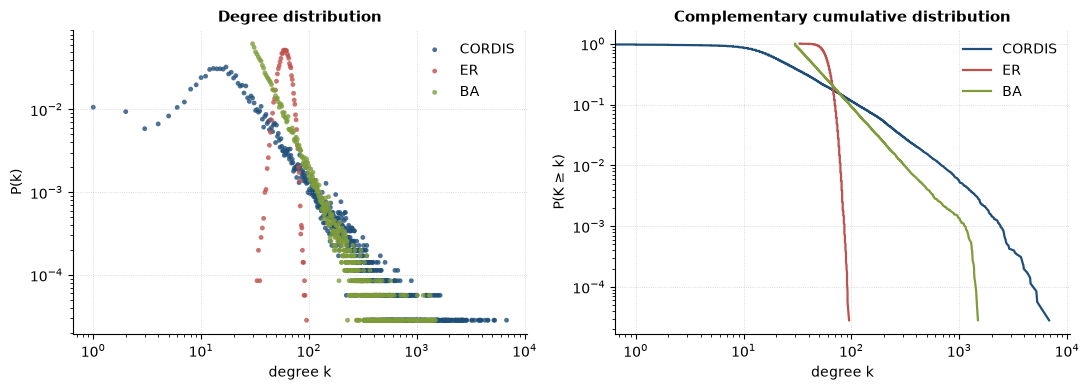
\includegraphics[width=0.86\textwidth]{degree_distribution.png}
\caption{Degree distribution of the three networks on log-log axes: the probability $P(k)$ that a node has $k$ partners (left), and the complementary cumulative distribution $P(K \ge k)$, the share of nodes with at least $k$ partners (right).}
\label{fig:degree}
\end{figure*}

A tail this heavy raises a familiar question: does the degree follow a power law, as preferential attachment would predict? To answer it, we fitted the tail following Clauset et al.~\cite{clauset2009}, with the \texttt{powerlaw} package~\cite{alstott2014}. The method passes a first test on the BA graph, where it recovers the theoretical exponent ($\alpha = 2.96$, over 52\% of the nodes). On CORDIS, by contrast, it returns $\alpha = 2.40$ only above $k = 172$, that is for a mere 6.6\% of the nodes, and even there a log-normal fits significantly better (log-likelihood ratio $R = -9.37$, $p = 0.004$). The distribution is heavy-tailed, then, but not scale-free in the strict sense.

This is precisely what the construction of the network would lead one to expect. An organisation does not gather its partners link by link, as in the BA model, but consortium by consortium: its degree is the number of distinct organisations it meets across its projects, and it therefore compounds the two skewed quantities described in Section~\ref{sec:data}, the number of projects and their size. For the 62.6\% of organisations with a single project, the degree is simply the size of that consortium minus one, and these organisations make up much of the body of the distribution. The tail, instead, belongs to organisations that take part in dozens of projects, often large ones, while a handful of hubs take part in hundreds or even more than a thousand.

\subsection{Components and Paths}

CORDIS is the only network that falls apart into pieces, though not by much. Outside the giant component remain only the isolated organisations and the minor components described in Section~\ref{sec:data}, each of them almost always a single consortium that shares no member with the rest. Inside the giant component, distances are remarkably short. The average path length is 2.72, lower than in both ER (2.90) and BA (2.82), so that two organisations picked at random are typically two or three steps apart. The hubs are largely responsible for this: linked to thousands of organisations each, they act as shortcuts that bring distant parts of the network within easy reach. The diameter, however, tells a different story, and is the largest of the three (6 against 4). The network is compact at its core, yet a few pairs of organisations remain farther apart than any pair in the two models, which points to a thin periphery of consortia attached to the rest through very few members.

\subsection{Clustering and Density}

\begin{figure}[t]
\centering
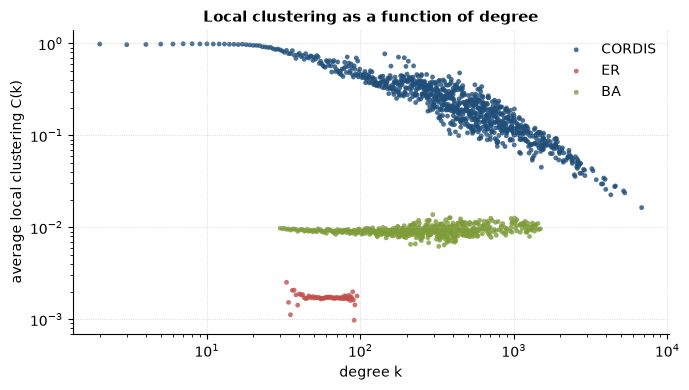
\includegraphics[width=0.95\columnwidth]{clustering_vs_degree.png}
\caption{Average local clustering coefficient of the nodes with degree $k$. In CORDIS it is close to 1 for the organisations with few partners, whose neighbours are the members of one consortium, and falls for the hubs.}
\label{fig:clustering}
\end{figure}

At first sight, CORDIS looks extraordinarily clustered. The three networks share the same density (0.0017), yet its average clustering coefficient reaches 0.78: about 460 times that of ER, where it equals the density just as theory predicts, and more than 80 times that of BA. Taken at face value, this would signal a remarkable inclination to close triangles. The explanation, however, lies in the data rather than in the organisations. Every project is a clique, so an organisation with a single project of three or more participants sees all its partners linked to one another, and scores a coefficient of exactly 1. High clustering is, in fact, a well-known property of projected bipartite networks~\cite{newman2001,opsahl2013}, and Figure~\ref{fig:clustering} makes it visible. The coefficient stays close to 1 for organisations with few partners, mostly those with one or a few projects, and then declines steadily, whereas in both models it remains flat. The transitivity, dominated as it is by the hubs, is accordingly far lower (0.13).

Here the comparison with ER and BA reaches its limit. Neither model contains projects, so neither can say how much of the clustering stems from shared membership and how much from a genuine preference for the partners of one's partners. This is the main weakness of the standard reference models for our data, and the reason why Section~\ref{sec:open} turns to a null model that keeps the projects.

\subsection{Centrality}

We computed six measures of centrality: degree, closeness, harmonic centrality, betweenness, PageRank and eigenvector centrality. However different their definitions, at the top they tell the same story. Thirteen organisations are enough to fill all six top-ten lists, and the Fraunhofer Society leads every one of them, with the Spanish CSIC and the French CNRS close behind. All thirteen are research organisations or universities. Private companies, by contrast, make up 58\% of the nodes, yet none of them reaches the core: they are the majority of the network and absent from its heart. The pattern is not new, since a core of universities and research organisations had already emerged in the first five Framework Programmes~\cite{roediger2008}.

\begin{table}[t]
\caption{Concentration of centrality in the top 1\% of nodes, and Spearman correlation with degree.}
\label{tab:centrality}
\small
\begin{adjustbox}{max width=\columnwidth}
\begin{tabular}{lrrrrrr}
\toprule
 & \multicolumn{3}{c}{Top 1\% share (\%)} & \multicolumn{3}{c}{$\rho$ with degree} \\
\cmidrule(lr){2-4}\cmidrule(lr){5-7}
 & CORDIS & ER & BA & CORDIS & ER & BA \\
\midrule
Betweenness & 73.9 & 1.8 & 47.0 & 0.74 & 1.00 & 0.96 \\
PageRank & 19.2 & 1.3 & 8.2 & 0.97 & 1.00 & 1.00 \\
Eigenvector & 18.5 & 1.4 & 10.0 & 0.86 & 0.99 & 0.80 \\
\bottomrule
\end{tabular}
\end{adjustbox}
\end{table}

Across the whole network, however, the six measures agree less than at the top, with rank correlations ranging from 0.69 to 1.00, and the way they part company is revealing. PageRank follows degree almost step by step. Betweenness does not ($\rho = 0.74$, against 0.96 in BA), and it is strikingly concentrated: the top 1\% of the organisations hold 73.9\% of it, against 47.0\% in BA and a mere 1.8\% in ER (Table~\ref{tab:centrality}). Once again, the construction is at work. An organisation whose partners are all linked to one another lies on no shortest path, and this is precisely the condition of every organisation with a single project. Brokerage is thus left to those that take part in many projects and, among them, to the few that bridge consortia with no other member in common. The Horizon Europe network, in the end, is held together by a small circle of research organisations and universities, while most companies enter it through a single project and remain at its edge.

\subsection{Degree Correlations}

Unlike the two models, which show no degree correlations, CORDIS is disassortative ($r = -0.102$~\cite{newman2002}): well-connected organisations tend, on average, to link to poorly connected ones. The effect is concentrated among the largest hubs, whose partners have, on average, far fewer partners than those of smaller organisations. It would be tempting to read this as hubs keeping their distance from one another, but the explanation is probably more mundane. In a simple graph two organisations can share at most one link, so hubs with thousands of partners cannot be connected to each other often enough to balance their many ties to small organisations. A negative coefficient can thus arise from the degree sequence alone~\cite{maslov2004,park2003}.

In short, the network is heavy-tailed, compact, and held together by a handful of hubs.

\section{Open Question}
\label{sec:open}

\subsection{Design}

Answering the research question requires three decisions: where to look, what to measure, and whom to compare.

\emph{Where: inside communities.} Global centrality is the wrong lens here. As Section~\ref{sec:analysis} shows, it is dominated by a dozen organisations, so a comparison between areas at that level would mostly tell us where those few are based. Collaboration, moreover, tends to cluster into groups, and the more telling question is who holds the centre of each one. Communities also offer a common scale: since positions are ranked within each community, they can be compared across communities of very different size.

\emph{What: internal degree.} The centrality of an organisation is measured by its internal degree, the number of its partners inside its own community, each counted once. We prefer this transparent measure to more elaborate ones because its meaning is unambiguous and its limits are easy to state. The main limit is that it is closely tied to participation, since every project brings partners; this is why the analysis then asks what remains once participation is taken into account.

From this measure we derive two quantities. The \emph{centrality percentile} of an organisation is its rank among the members of its community, from 0 to 1, so that positions can be compared across communities. The \emph{centre} of a community is the 1\% of its members with the highest internal degree. Only communities with at least 1,000 members are analysed, so that every centre counts at least ten organisations.

\emph{Who: five areas.} Countries are grouped into the four European regions of the United Nations geoscheme~\cite{m49}, namely Western, Northern, Southern and Eastern Europe, with Cyprus and Kosovo assigned to Southern Europe. All other countries form a fifth group, the rest of the world, led in size by the United States, Turkey, China and Israel.

\subsection{A Null Model that Keeps the Projects}

ER and BA tell how far the network is from randomness, but they cannot answer our question. In both, links form one at a time between anonymous nodes, whereas here links come in blocks, one consortium at a time, and every organisation has its own participation. To tell whether an area is central because of how much its organisations participate or for some other reason, the baseline must keep both the projects and the participation of each organisation. We therefore build null networks by reassigning the organisations to the participations at random, within classes of project size (2, 3, 4--5, 6--9, 10--19, 20--49, 50 or more participants), and then projecting them exactly as the observed data. What an organisation brings to the programme, namely how much it participates and in consortia of which size, is preserved; with whom it participates becomes random and, in particular, independent of its country. The size classes matter, because the number of partners gained from a project depends on the size of the consortium, which a model keeping only the number of projects would randomise. An organisation drawn twice into the same project is counted once, so the constraints hold almost exactly: 95.7\% of the projects and 99.2\% of the organisations keep their numbers unchanged.

In a null network, two organisations with the same participation are equally likely to be central, wherever they are based: the null networks thus show what participation alone would produce. We generated twenty of them, and on each we ran the community detection and the comparison by area. Observed values are compared with the mean and the range of the twenty. A value just outside this range is weak evidence, since even a network drawn from the null model itself would fall outside the range of twenty others about one time in ten. Only large deviations are therefore interpreted.

\subsection{Communities}

\begin{table}[t]
\caption{Communities found by three algorithms on the weighted network. A community is large if it has at least 1,000 members. Coverage is the share of organisations in large communities, and conductance is averaged over them. The last row shows the mean modularity of Louvain on the twenty null networks.}
\label{tab:communities}
\small
\setlength{\tabcolsep}{4pt}
\begin{adjustbox}{max width=\columnwidth}
\begin{tabular}{lrrrrr}
\toprule
 & Communities & Large & Coverage (\%) & Modularity & Conductance \\
\midrule
Louvain (best of 10) & 72 & 7 & 90.3 & 0.414 & 0.43 \\
Infomap & 1,046 & 2 & 20.9 & 0.342 & 0.47 \\
Label Propagation & 160 & 1 & 95.3 & 0.032 & 0.01 \\
\midrule
Null networks (Louvain) & & & & 0.202 & \\
\bottomrule
\end{tabular}
\end{adjustbox}
\end{table}

Communities were detected on the weighted network with the \texttt{igraph} implementations of three algorithms, each embodying a different idea of what a community is: Louvain~\cite{blondel2008}, which maximises modularity; Infomap~\cite{rosvall2008}, which follows the flow of a random walk; and Label Propagation~\cite{raghavan2007}, in which every node adopts the label most common among its neighbours. Table~\ref{tab:communities} compares them through the modularity of each partition and the average conductance of its large communities~\cite{yang2015}. 

The three pictures differ. Label Propagation gathers 95.3\% of the organisations into a single community, as one would expect in a network this dense, where labels can travel through the hubs. Infomap, at the other extreme, returns more than a thousand communities, only two of them large, and agrees with Louvain only in part (NMI~\cite{danon2005} of 0.41). Louvain, repeated ten times with different seeds and taken at its highest modularity ($Q = 0.414$), divides 90.3\% of the organisations into seven large communities, and this is the partition we use. The choice is instrumental rather than a claim that these are the true communities, and three checks help qualify it.

\begin{table}[t]
\caption{The seven large communities of the reference partition, named after their most connected member and numbered from the largest to the smallest as in Figure~\ref{fig:centres}. W, N, S and E stand for Western, Northern, Southern and Eastern Europe, and RoW for the rest of the world.}
\label{tab:seven}
\small
\renewcommand{\arraystretch}{1.15}
\setlength{\tabcolsep}{4pt}
\begin{adjustbox}{max width=\columnwidth}
\begin{tabular}{@{}lrrrrrrr@{}}
\toprule
 & & & \multicolumn{5}{c}{Members by area (\%)} \\
\cmidrule(l){4-8}
Community & Size & Conductance & W & N & S & E & RoW \\
\midrule
1 CERTH (EL) & 7,540 & 0.39 & 29.6 & 16.4 & 39.8 & 9.4 & 4.8 \\
2 CNRS (FR) & 6,672 & 0.47 & 35.9 & 16.0 & 21.3 & 9.0 & 17.7 \\
3 Fraunhofer (DE) & 5,171 & 0.45 & 44.7 & 18.3 & 25.0 & 5.3 & 6.7 \\
4 Wageningen (NL) & 4,372 & 0.43 & 29.2 & 14.7 & 33.1 & 10.3 & 12.7 \\
5 INSERM (FR) & 4,123 & 0.39 & 36.8 & 19.2 & 21.8 & 6.1 & 16.2 \\
6 HCMR (EL) & 2,000 & 0.51 & 23.4 & 22.8 & 32.5 & 13.4 & 8.0 \\
7 Indra (ES) & 1,159 & 0.36 & 45.6 & 12.0 & 28.6 & 9.1 & 4.7 \\
\midrule
All seven & 31,037 & & 34.6 & 17.0 & 29.1 & 8.6 & 10.7 \\
\bottomrule
\end{tabular}
\end{adjustbox}
\end{table}

\emph{Stability.} The ten Louvain partitions have almost the same modularity (0.408--0.414) and six to eight large communities, but agree with the reference only moderately (NMI between 0.50 and 0.60): organisations are assigned differently from one run to the next.

\emph{Separation.} In every large community more than a third of the links of the members lead outside (conductance from 0.36 to 0.51, Table~\ref{tab:seven}).

\emph{Significance.} The null networks, where partners are random, reach a modularity of 0.202 (0.199--0.204). Half of the observed modularity is therefore produced by the construction alone, and only the other half reflects how partners are chosen.

The communities are therefore real but blurred, and we treat them as a lens rather than as objects. One property makes them well suited to our question: they do not follow geography. Their agreement with the country of the organisations is NMI $= 0.054$, and with the area 0.025, above the null values (0.017 and 0.001) but still close to zero. Every large community includes all five areas (Table~\ref{tab:seven}): Southern Europe, for instance, ranges from 21\% to 40\% of the members. Three of the seven hubs, namely Wageningen University, the French National Institute of Health and Medical Research (INSERM) and the Hellenic Centre for Marine Research (HCMR), are specialised institutes, which suggests that communities may form around research fields. The other hubs, however, are generalist research organisations or, in the case of Indra, a company, and since project topics were not collected, this reading cannot be tested here. Ultimately, what matters for our question is that every area is present in every community, so it makes sense to ask which areas hold the centre.

\subsection{Who Holds the Centre}

\begin{table}[t]
\caption{The five areas in the seven large communities. The first three columns give the percentage of each area among all members, among the most active organisations and among the central ones. In each community, the most active are the 1\% of members with the most projects, and the central the 1\% with the most partners inside the community. The ratio divides the third percentage by the first. The centrality gap is 0 when the organisations of an area are as central as others with the same number of projects.}
\label{tab:regions}
\small
\renewcommand{\arraystretch}{1.15}
\setlength{\tabcolsep}{5pt}
\begin{adjustbox}{max width=\columnwidth}
\begin{tabular}{@{}lrrrrrr@{}}
\toprule
 & \multicolumn{3}{c}{Share of the area (\%)} & & \multicolumn{2}{c}{Centrality gap} \\
\cmidrule(lr){2-4}\cmidrule(l){6-7}
 & Members & Most active & Central & Ratio & CORDIS & Null model \\
\midrule
Western Europe & 34.6 & 36.7 & 39.2 & 1.13 & $+0.007$ & $+0.004$ \\
Northern Europe & 17.0 & 19.3 & 17.4 & 1.02 & $-0.007$ & $+0.003$ \\
Southern Europe & 29.1 & 40.5 & 37.3 & 1.28 & $0.000$ & $+0.003$ \\
Eastern Europe & 8.6 & 3.2 & 5.1 & 0.60 & $+0.014$ & $+0.006$ \\
Rest of the world & 10.7 & 0.3 & 1.0 & 0.09 & $-0.024$ & $-0.030$ \\
\bottomrule
\end{tabular}
\end{adjustbox}
\end{table}

Together, the seven large communities count 31,037 organisations, and 311 of them make up the centres. Table~\ref{tab:regions} sets the weight of each area among all members against its weight among the central organisations.

The two do not match. Southern Europe is the most over-represented area, rising from 29.1\% of the members to 37.3\% of the central organisations (a ratio of 1.28), and Western Europe follows at some distance (1.13), while Northern Europe holds the centre roughly in proportion to its size (1.02). At the other end, Eastern Europe falls from 8.6\% of the members to 5.1\% of the central organisations (0.60), and the rest of the world almost vanishes, with just 3 central organisations out of 311. Since the partition is unstable, the comparison was repeated on all ten Louvain partitions. Every imbalance keeps its direction, with one exception: Northern Europe, whose ratio wavers between 0.97 and 1.13. The reference partition, moreover, is close to the most favourable case for Eastern Europe, whose ratio ranges from 0.28 to 0.61.

\begin{figure}[t]
\centering
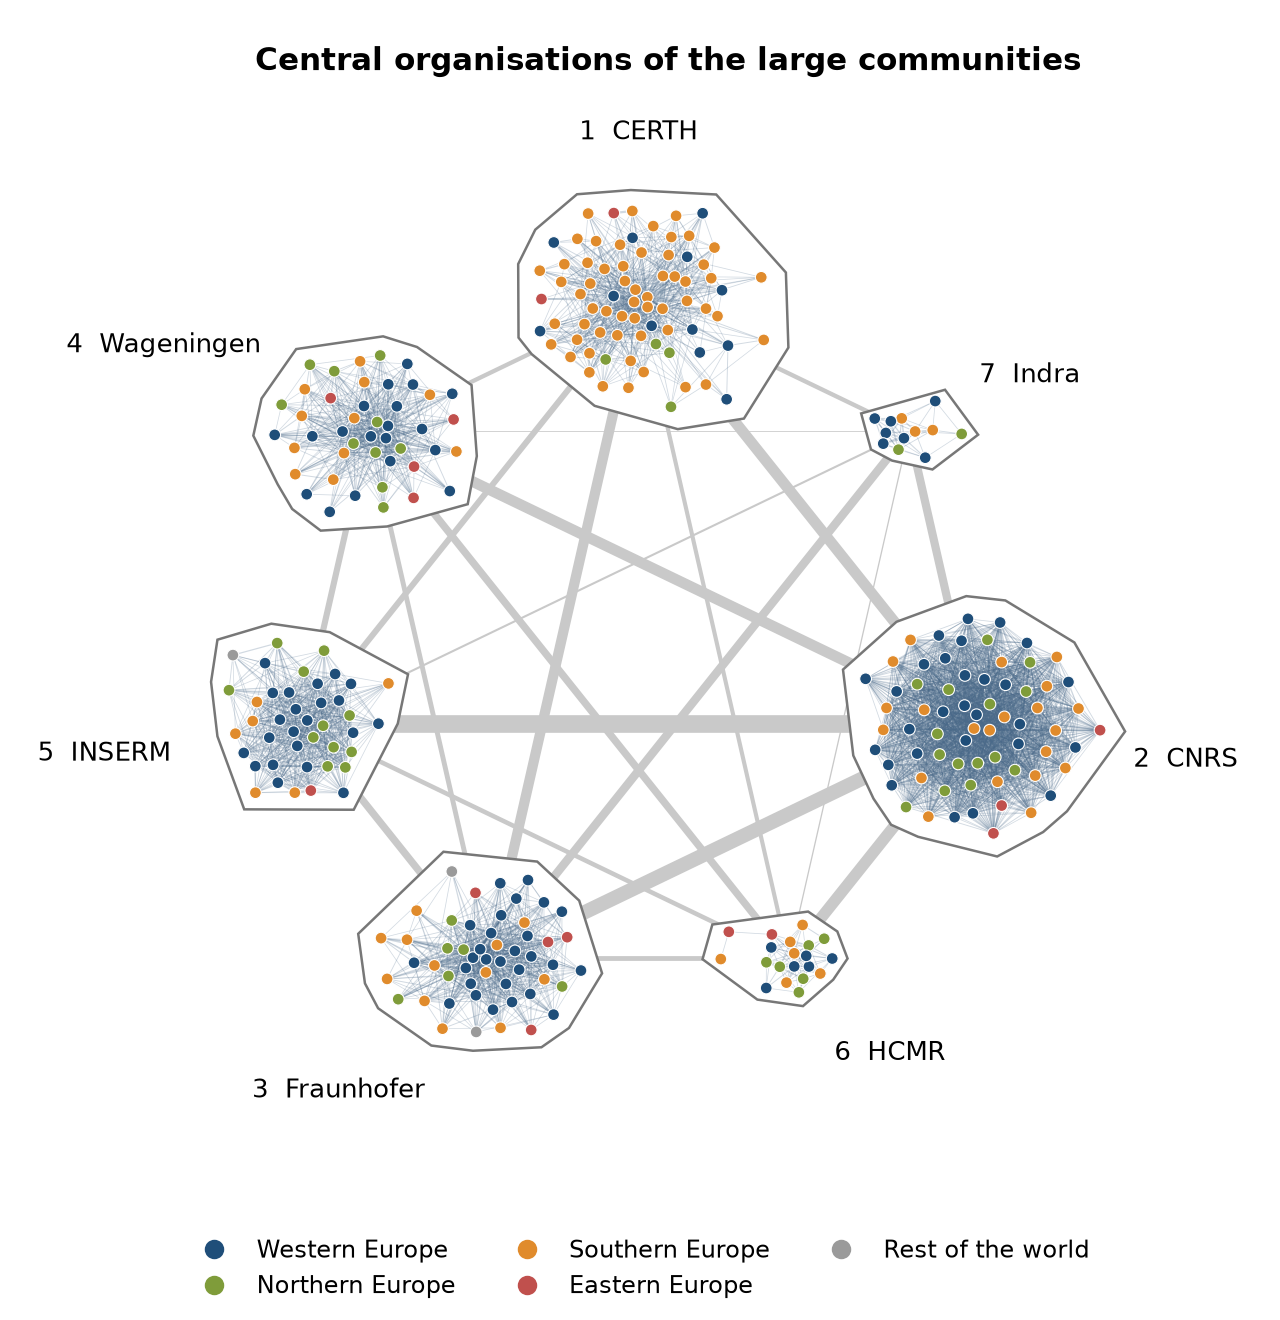
\includegraphics[width=0.95\columnwidth]{central_organisations_by_community.png}
\caption{The central organisations of the seven large communities, coloured by area and grouped by community. Thicker lines between groups mean more links between their central organisations.}
\label{fig:centres}
\end{figure}

The excess of Southern Europe, however, is far from spread across the network (Figure~\ref{fig:centres}). In the reference partition it comes almost entirely from a single community, the largest, whose hub is CERTH: here 57 of the 75 central organisations are Southern European. Take this community away, and the picture changes. In the other six together, Southern Europe holds 59 of the 236 central organisations, about a quarter, which is close to its weight among their members. Their centres are mixed, or led by Western Europe, as in the communities of Fraunhofer and INSERM. The percentages by area, in other words, are averages of centres with very different compositions, and the excess of Southern Europe is the signature of one community rather than a feature of the network as a whole. It is tempting to conclude that the composition of a centre follows the organisation around which the community forms, and the reading is plausible, but a single partition cannot establish it.

\subsection{The Role of Participation}

One question is still open: do these imbalances reflect the position of each area in the network, or simply how much its organisations participate? Participation is expected to weigh heavily, since internal degree is closely tied to it. What matters is what remains once participation is taken into account, and three pieces of evidence, of increasing strength, all point in the same direction.

\emph{The imbalance is already visible in participation.} A first sign comes from defining the centre of each community by projects rather than by links, as the 1\% of members with the most projects. The picture barely changes, and for three areas it becomes even sharper (Table~\ref{tab:regions}): Eastern Europe falls to 3.2\% of these most active organisations and the rest of the world to 0.3\%, while Southern Europe rises to 40.5\%. Centrality and participation, however, are related without being the same thing: their rank correlation is 0.65, and 71\% of the central organisations are also among the most active of their community. Their overlap alone, then, cannot settle the question.

\emph{At equal participation, areas are almost equally central.} A sharper test compares like with like. Organisations were grouped by number of projects, and within each group the average centrality percentile of each area was computed. The four European areas turn out to be almost indistinguishable: their averages never differ by more than 0.03, and Eastern Europe is never the lowest of the four. What Eastern Europe lacks, then, is not centrality but very active organisations: only 0.4\% of them (11 out of 2,660) take part in fifty projects or more, against 1.2\% in Western and Southern Europe. The rest of the world is the only exception, falling below the others at every number of projects.

\begin{figure}[t]
\centering
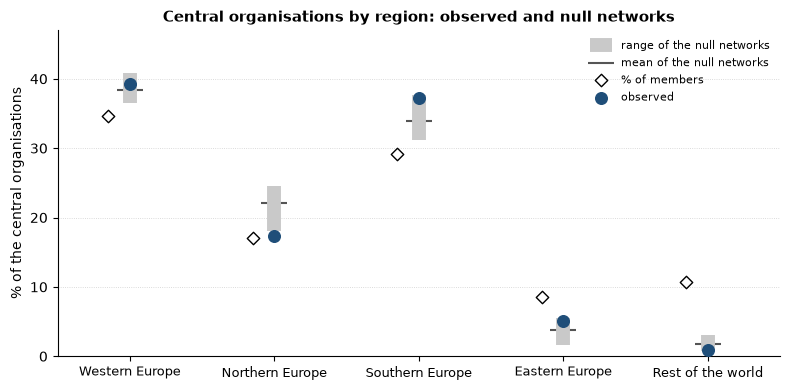
\includegraphics[width=\columnwidth]{central_organisations_by_region_vs_null.png}
\caption{Share of the central organisations in each area: CORDIS, and mean and range of the twenty null networks, where partners are assigned ignoring the country. Only Northern Europe falls outside the range.}
\label{fig:regions}
\end{figure}

\emph{The null model reproduces both.} The strongest test asks whether participation alone would produce these results. Averaging the differences above gives, for each area, a \emph{centrality gap} at equal number of projects (Table~\ref{tab:regions}), and for every area the observed gap lies within 0.01 of the null mean. The null range is very narrow, and four areas fall just outside it, but by 0.004 at most. The rest of the world, by contrast, lies within it: its negative gap ($-0.024$) is close to what the null networks produce ($-0.030$ on average). Its organisations are therefore less central than others with as many projects because of how they participate, which the null model preserves down to the size of their consortia, and not because of whom they participate with.

The share of central organisations tells the same story (Figure~\ref{fig:regions}). Four areas out of five are within the range of the null networks, including Eastern Europe, whose observed 5.1\% is, if anything, on the high side of what participation would give. Only Northern Europe falls outside, with fewer central organisations than in any null network (17.4\%, against a minimum of 18.0\%).

\subsection{Countries}

\begin{figure}[t]
\centering
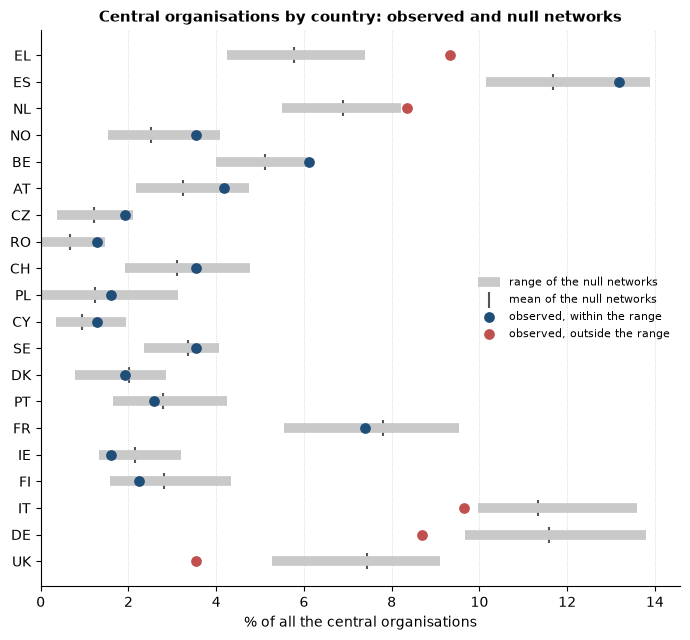
\includegraphics[width=0.92\columnwidth]{central_organisations_by_country_vs_null.png}
\caption{Share of the central organisations in each country, for the countries that hold at least 1\% of them: CORDIS against the twenty null networks, sorted by the difference from the null mean. Greece stands out above its range, the United Kingdom and Germany below.}
\label{fig:countries}
\end{figure}

Repeating the last comparison by country shows where the residuals lie (Figure~\ref{fig:countries}). Of the twenty countries with at least 1\% of the central organisations, five are outside the null range, where about two would be expected by chance, and three deviations are large. Greece has 9.3\% of the central organisations against 5.8\% in the null networks (maximum 7.4\%). The United Kingdom has 3.5\% against 7.4\% (minimum 5.3\%), about half of what its participation would give, and Germany 8.7\% against 11.6\% (minimum 9.7\%), three quarters. These three countries account for the residuals of the areas. The United Kingdom explains most of the shortfall of Northern Europe (3.9 of 4.7 percentage points) and Greece the whole excess of Southern Europe over its null mean (3.6 against 3.4), while the shortfall of Germany is offset, within Western Europe, by the Netherlands, Belgium and Austria.

\section{Discussion}
\label{sec:discussion}
\subsection{Answer to the Research Question}

The most central organisations are not evenly distributed across areas, but most of the imbalance mirrors differences in participation. Organisations that take part in the same number of projects are almost equally central wherever they are based in Europe, and a model that knows nothing about countries reproduces the under-representation of Eastern Europe and of the rest of the world, as well as most of the over-representation of Southern Europe. At equal participation, in other words, no further disadvantage emerges for any area as a whole, except a small shortfall in Northern Europe that comes from a single country. What participation does not explain is concentrated in a few countries, discussed below.

This is a negative result, but an informative one, because it was far from guaranteed. Had position mattered, an Eastern European organisation with twenty projects would have been less central than a Western one with as many, and the data could easily have shown it. If anything, they show the opposite. What sets Eastern Europe apart is participation itself, and in particular the scarcity of organisations that take part again and again: its weight falls from 8.6\% of the members to 3.2\% of the most active.

These results bear, with due caution, on how the geographic gap is understood. They suggest that efforts to broaden participation address the main source of the imbalance, and they offer no evidence that organisations from these areas, once they take part, end up at the margins of collaboration. They cannot say, however, why participation is lower in the first place: that depends on factors a co-participation network does not record, and possibly on the network itself, if being less connected also means being invited into fewer consortia.

\subsection{Two Unexpected Findings}

The first is the geography of the core. Greece is one of the fifteen widening countries of Horizon Europe~\cite{widening}, yet it ranks third for central organisations, after Spain and Italy and ahead of Germany, with about a third as many linked organisations as Germany (1,215 against 3,484). The communities offer a likely explanation. Two of the seven large ones, including the largest, have a Greek organisation as their most connected member (Table~\ref{tab:seven}): the Centre for Research and Technology Hellas (CERTH), which is also the fourth broker of the whole network by betweenness, and the Hellenic Centre for Marine Research. The community of CERTH is also the one whose centre accounts for almost the whole excess of Southern Europe. A plausible reading is that being the hub of a community draws other organisations of the same country towards its centre, which the same participation, spread over communities led by others, would not do. Whatever the mechanism, the label of widening country covers very different situations: by this measure Greece belongs to the core of the programme, while the six Member States of our Eastern European group, all of them widening countries, do not.

The second is the shortfall of the United Kingdom and of Germany. For the United Kingdom an institutional explanation is at hand, which we offer as a hypothesis. For the calls of 2021--2023, British organisations took part in Horizon Europe under a transitional arrangement, mostly as associated partners funded by a national guarantee and, as a rule, unable to coordinate projects. The country became associated to the programme only on 1 January 2024~\cite{ukassociation}. This status may have shaped which consortia British organisations could join, and therefore how many of their partners they share with the rest of their community. Testing this would require separating the projects of the two periods and the roles of the participants, which we have not done. For Germany we have no firm explanation. One candidate is mechanical: since the centre is a fixed share of each community, a country whose most active organisations are concentrated in the same communities ends up competing with itself for the same positions.

\subsection{Limitations}

\emph{Participation is not independent of position.} The null model takes the participation of each organisation as given. If peripheral organisations are invited into fewer consortia, as studies of earlier programmes suggest~\cite{enger2018}, part of what this report attributes to participation would itself be an effect of position. Separating the two would require following organisations over time, across programmes.

\emph{One partition.} The comparison by area was repeated on ten Louvain partitions, but the comparisons with the null networks and the analysis by country rest on the reference partition, in a network whose communities are blurred.

\emph{Centrality as presence.} The internal degree counts partners. It follows participation closely and says nothing about the role played in a project: it measures presence, not leadership. Comparing how often the organisations of each area coordinate their projects, which the roles recorded in CORDIS would allow, is a natural next step.

\emph{What the null model keeps.} The number and the size class of the projects of each organisation, but not their topic or funding instrument. The deviations of Greece, the United Kingdom and Germany show what participation does not explain, not its cause.

\emph{Small numbers.} The centres contain 311 organisations, 16 of them in Eastern Europe and 3 in the rest of the world, and only 11 and 5 organisations of these areas have fifty projects or more. Twenty null networks give a range, not a test: values close to its limits should not be over-interpreted.

\emph{Arbitrary thresholds.} The centre is the top 1\% of a community, and communities below 1,000 members are excluded. Other thresholds were not examined.

\emph{Areas and time.} The European regions come from an external classification, and the rest of the world mixes associated and third countries. The programme is still running, the most recent years are incomplete, and the analysis is a single snapshot.

\subsection{Conclusion}

In the collaboration network of Horizon Europe, the centre of the communities is unevenly distributed across Europe, but at equal participation organisations are almost equally central wherever they are based. The imbalance is visible first in how much each area takes part in the programme, and only a few countries, Greece above all, and the United Kingdom and Germany in the opposite direction, deviate from what their participation would give. Reaching these conclusions required a null model built for a projected network, without which much of the structure described here would have been mistaken for a property of the organisations. Two extensions would test the open points: following the network over the years of the programme, to see whether the position of British organisations changed with association, and adding the topics of the projects, to verify what the communities stand for.

\bibliographystyle{ACM-Reference-Format}
\bibliography{biblio}

\end{document}
